\documentclass[12pt, a4paper, oneside, openright]{Thesis} % Paper size, default font size and one-sided paper
\usepackage[utf8]{inputenc}
\usepackage{wrapfig}
\usepackage{lscape}
\usepackage{rotating}
\usepackage{graphicx}
\usepackage{caption}
\usepackage{amsmath, nccmath}
\usepackage{comment}
\usepackage{afterpage}
\usepackage{multirow}
\usepackage{multicol}
\usepackage{cleveref}
\usepackage{rotating}
% \usepackage[font=small]{caption}
% \captionsetup{compatibility=false}
% \usepackage{subcaption}
% \usepackage{subfig}
\usepackage[square,sort,comma,numbers]{natbib}
\usepackage{makecell}
\usepackage{booktabs}
\usepackage{multirow}
\usepackage{lscape}
\usepackage{longtable}
\usepackage{placeins}
\usepackage{adjustbox}
\usepackage{arydshln} % dashed midline
\usepackage{ragged2e}
\usepackage{lipsum}
\usepackage{mathtools} % To use box inside an aligned environment
\usepackage{enumitem} % for roman letter lists
% \usepackage{subfig}


\newcommand\myemptypage{
    \null
    \thispagestyle{empty}
    \addtocounter{page}{-1}
    \newpage
    }
%\usepackage[width=14cm, left=3cm]{geometry}

% prints author names as small caps


%\usepackage{subcaption} %incompatible with subfig
\graphicspath{{Pictures/}} % Specifies the directory where pictures are stored

%\usepackage[square, numbers]{natbib} % Use the natbib reference package - read up on this to edit the reference style; if you want text (e.g. Smith et al., 2012) for the in-text references (instead of numbers), remove 'numbers' v
%\bibliographystyle{abbrvnat}
%\setcitestyle{authoryear,open={((},close={))}}
\hypersetup{urlcolor=blue, colorlinks=true} % Colors hyperlinks in blue - change to black if annoyingv`	
\title{\ttitle} % Defines the thesis title - don't touch this




%%%% New added


\usepackage{tikz}
\usetikzlibrary{shapes.geometric, arrows}

% Defining Tickz Style
\tikzstyle{startstop} = [rectangle, rounded corners, minimum width=3cm, minimum height=1cm, text centered, text width = 10cm, draw=black, fill=white]

% \tikzstyle{startstop1} = [rectangle, rounded corners, minimum width=3cm, minimum height=1cm, text centered, draw=black, fill=white, text width = 10cm]

% \tikzstyle{io} = [trapezium, trapezium left angle=70, trapezium right angle=110, minimum width=3cm, minimum height=1cm, text centered, text width = 4.5cm, draw=black, fill=blue!30]

\tikzstyle{process} = [rectangle, minimum width=3cm, minimum height=1cm, text centered, text width = 6cm, draw=black, fill=white, text width = 10cm]

% \tikzstyle{decision} = [diamond, minimum width=3cm, minimum height=1cm, text centered, draw=black, fill=green!30]

\tikzstyle{arrow} = [ultra thick,->,>=stealth]







\usepackage[T1]{fontenc}

\begin{document}
% \makeatletter
% \renewcommand*{\NAT@nmfmt}[1]{\textsc{#1}}
% \makeatother

% prints author names as small caps
% it is sometimes necessary in user documents to have access to such package-internal macros, and so the commands \makeatletter and \makeatother change the catcode 


%\frontmatter % Use roman page numbering style (i, ii, iii, iv...) for the pre-content pages

\setstretch{1.6} % Line spacing of 1.6 (double line spacing)

% Define the page headers using the FancyHdr package and set up for one-sided printing
\fancyhead{} % Clears all page headers and footers
\rhead{\thepage} % Sets the right side header to show the page number
\lhead{} % Clears the left side page header

\pagestyle{fancy} % Finally, use the "fancy" page style to implement the FancyHdr headers

\newcommand{\HRule}{\rule{\linewidth}{0.5mm}} % New command to make the lines in the title page

% PDF meta-data
\hypersetup{pdftitle={\ttitle}}
\hypersetup{pdfsubject=\subjectname}
\hypersetup{pdfauthor=\authornames}
\hypersetup{pdfkeywords=\keywordnames}




% --------------------------------------------------





%----------------------------------------------------------------------------------------
%	TITLE PAGE
%----------------------------------------------------------------------------------------
\begin{comment}
\begin{titlepage}
\begin{center}

\HRule \\[0.4cm] % Horizontal line
{\huge \bfseries \ttitle}\\[0.4cm] % Thesis title
\HRule \\[1.5cm] % Horizontal line
 
\large \textit{A thesis submitted in fulfillment of the requirements\\ for the degree of \degreename}\\[0.3cm] % University requirement text
\textit{by}\\[0.4cm]

%\href{http://home.iitk.ac.in/~saiwal}{\authornames}

\vfill
\graphicspath{ {./Figures/} }
\begin{figure}[hb]
  \centering
  \includegraphics[width=0.4\linewidth]{Images/redlogo.png}
\end{figure}

\DEPTNAME\\ % Research group name and department name
\textsc{ \UNIVNAME}\\[1.5cm] % University name
\large \today\\[2cm] % Date


\end{center}

\end{titlepage}
\end{comment}
%\begin{document}
%\begin{titlepage}


%\include{title1}
%\end{titlepage}
%\myemptypage
%\afterpage{\null\newpage}
%\include{blank_page_1}
%\newpage
%\newpageer
%\newgeometry{centering,top = 2.54cm,bottom = 2.54cm,left = 2.54cm, right = 2.54cm, includeheadfoot}

\pagenumbering{gobble}% Remove page numbers (and reset to 1)
\thispagestyle{empty}
\singlespacing
\begin{titlepage}

\begin{center}
%\begin{minipage}{0.75\linewidth}
    \centering
     
%=====================================================%
%---------------THESIS TITLE--------------------------%
%=====================================================%    
\definecolor{blue}{rgb}{0,0,1} % before using a colour one has to define it like this, here you have given color with rgb as 0,0,1 as blue
      
  {{\LARGE \textbf{Thesis Title}\par}}
    \vspace{0.8cm}% FOR CREATING DESIRED SPACE BETWEEN THE LINES
     
%=====================================================%
%---------------Partial Fulfillment---------------------%
%=====================================================%
  \vspace{0.4cm}
    \textbf{ {A Project Report Submitted\\ In Partial Fulfilment of the Requirements\\ for the Degree of \\}}
    \vspace{0.8cm}
    {
   \textsc{\textbf{\large Bachelor of Technology\\}} \par}
   \textbf{\Large in\\} \par
   \textsc{\textbf{\large Computer Science \& Engineering}} \par
    \vspace{0.3cm}

%=====================================================%
%---------------AUTHOR'S NAME-------------------------%
%=====================================================%

    {\large by\par}
    \vspace{0.3cm}
    {\textbf{{Name} (Roll No. 00000000000)}}\\
    {\textbf{{Name} (Roll No. 00000000000)}}\\
    {\textbf{{Name} (Roll No. 00000000000)}}\\
    \vspace{1.2cm}
    
%=====================================================%
%---------------Supervisor Name---------------------%
%=====================================================%    
%    {\Large \textbf{Doctor of Philosophy} \par}
%    \vspace{0.5cm}
    \textbf{ Under the Guidance of \\}
    {\textbf{{Prof. Name}}\\}
    
%    {\Large \textbf{(2013MEZ8469)}\par}
     \vspace{1.5cm}

%=====================================================%
%---------------UNIVERSITY lOGO-----------------------%
%=====================================================%

\includegraphics[width=0.2\linewidth]{ietlogo.png}
%    \rule{0.4\linewidth}{0.15\linewidth}\par
     \vspace{0.8 cm}

    
%=====================================================%
%---------------DEPARTMENT'S NAME-------------------------%
%=====================================================%
      
    
\textbf{{\large Department of Computer Science and Engineering\\}}

\vspace{0.1cm}
\textbf{{\Large Institute of Engineering \& Technology\\}}
  \vspace{0.1cm}
{\large\textsc{\textbf{Dr. APJ Abdul Kalam Technical University, Uttar Pradesh\\ }}}  

\vspace{1.6cm}

%=====================================================%
%---------------DATE----------------------------------%
%=====================================================%
   \textbf{ {\large {December, 2024}}}
%\end{minipage}

\end{center}
\end{titlepage}

%----------------------------------------------------------------------------------------
% Approval page
%----------------------------------------------------------------------------------------


%-------------------------------------------------------------
%	DECLARATION PAGE
%	Your institution may give you a different text to place here
%----------------------------------------------------------------------------------------

% ------------------------------------------------
% Professor's declaration


%------------------------------------------------------------------

%-------------------------------------------------------------
%	DECLARATION PAGE
%	Your institution may give you a different text to place here
%----------------------------------------------------------------------------------------

% ------------------------------------------------
% Professor's declaration

%\Certificate{\addtocontents{toc}{} %\begin{center}

%This is to certify that the project report entitled: \textbf{"Name of the Title"} submitted by \textbf{Your Name1, Your Name2, Your Name3} in the partial fulfillment for the award of the degree of Bachlor of Technology in Computer Science \& Engineering is a record of the bonafide work carried out by them under my supervision and guidance at the Department of Computer Science \& Engineering at Institute of Engineering \& Technology Lucknow.
%\par
%The project report has reached the standards fulfilling the requirements of the regulations related to the award of the degree.

%\par It is also certified that this work has not been submitted any where else for the award of any other degree to the best of my knowledge.
%\bigskip
%\bigskip
%\bigskip
%\bigskip


%\vspace*{2.5cm} %\vfill
%\begin{multicols}{2}
%\begin{center}
%\begin{flushleft}
%Date:
%\end{flushleft}
%\textbf{Prof. Akhilesh Kumar Maurya}\\
%Department of Civil Engineering,\\
%Indian Institute of Technology Guwahati.
%\end{center}
%\begin{flushleft}
%\begin{flushleft}
%Date:
%\end{flushleft}
%\ldots \ldots \ldots \ldots \ldots \ldots \ldots \ldots \ldots \ldots \ldots \ldots\\
%\textbf{(Prof. Name)}\\
%Department of Computer Science and Engineering,\\
%Institute of Engineering \& Technology, Lucknow
%\end{flushleft}
%\end{multicols}
%\vfill{}}


%\clearpage % Start a new page


%\Declaration{\addtocontents{toc}{} %\begin{center} % Add a gap in the Contents, for aesthetics

%We hereby declare that this submission of project is our own work and that to the best of our knowledge and belief it contains no material previously published or written by another person or material which to a substantial extent has been accepted for award of any other degree of the university or other institute of higher learning, except where due acknowledgement has been made in the text. \par
%This project report has not been submitted by us to any other institute for requirement of any other degree.
%\bigskip
%\bigskip
%\bigskip
%\bigskip

%This is to certify that the thesis entitled \textbf{``Thesis Title''}, submitted by \textbf{Your Name} to the Institute of Engineering \& Technology Lucknow, for the award of the degree of \textbf{Bachlor of Technology} in Transportation System Engineering, is a record of the original, bona fide research work carried out by him under our supervision and guidance. The thesis has reached the standards fulfilling the requirements of the regulations related to the award of the degree.

%\par The results contained in this thesis have not been submitted in part or in full to any other University or Institute for the award of any degree or diploma to the best of our knowledge.
%\bigskip
%\bigskip
%\bigskip
%\bigskip


%\vspace*{2.5cm} %\vfill

%\begin{multicols}{2}
%\begin{center}
%\begin{flushleft}
%Date:
%\end{flushleft}
%\textbf{Prof. Akhilesh Kumar Maurya}\\
%Department of Civil Engineering,\\
%Indian Institute of Technology Guwahati.
%\end{center}
%\begin{flushleft}
%\begin{flushleft}
%Date:
%\end{flushleft}
%\ldots \ldots \ldots \ldots \ldots \ldots \ldots \ldots \ldots \ldots \ldots \ldots\\

%\textbf{Signature of the Students}\\
 %\vspace{1.0 cm}
%Name (Roll Number)\\
%\vspace{1.0 cm}
%Name (Roll Number)\\
%\vspace{1.0 cm}
%Name (Roll Number)\\
%\end{flushleft}
%\end{multicols}
%\vfill{}}

%\clearpage


%\Certificate{\addtocontents{toc}{} %\begin{center} % Add a gap in the Contents, for aesthetics

%This is to certify that the project report entitled: \textbf{Name of the Title} submitted by \textbf{Your Name1, Your Name2 and Your Name3} in the partial fulfillment for the award of the degree of Bachelor of Technology in Computer Science \& Engineering is a record of the bonafide work carried out by them under our supervision and guidance at the Department of Computer Science \& Engineering, Institute of Engineering \& Technology Lucknow.


%\par It is also certified that this work has not been submitted any where else for the award of any other degree to the best of our knowledge.
%\bigskip
%\bigskip
%\bigskip
%\bigskip

%This is to certify that the thesis entitled \textbf{``Thesis Title''}, submitted by \textbf{Your Name} to the Institute of Engineering \& Technology Lucknow, for the award of the degree of \textbf{Bachlor of Technology} in Transportation System Engineering, is a record of the original, bona fide research work carried out by him under our supervision and guidance. The thesis has reached the standards fulfilling the requirements of the regulations related to the award of the degree.

%\par The results contained in this thesis have not been submitted in part or in full to any other University or Institute for the award of any degree or diploma to the best of our knowledge.
%\bigskip
%\bigskip
%\bigskip
%\bigskip


%\vspace*{2.5cm} %\vfill

%\begin{multicols}{2}
%\begin{center}
%\begin{flushleft}
%Date:
%\end{flushleft}
%\textbf{Prof. Akhilesh Kumar Maurya}\\
%Department of Civil Engineering,\\
%Indian Institute of Technology Guwahati.
%\end{center}
%\begin{flushleft}
%\begin{flushleft}
%Date:
%\end{flushleft}
%\ldots \ldots \ldots \ldots \ldots \ldots \ldots \ldots \ldots \ldots \ldots \ldots\\

%\hspace{2.0 cm}\textbf{(Co-supervisor Name)}\\
%Department of Computer Science and Engineering,\\
%Institute of Engineering \& Technology, Lucknow 

%\end{multicols}
%\vspace{2 cm}
%\hspace{2.0 cm}\textbf{(Supervisor Name)}\\
%Department of Computer Science and Engineering,\\
%Institute of Engineering \& Technology, Lucknow 
%\end{flushleft}
%\vfill{}}


%\clearpage % Start a new page


%----------------------------------------------------------------------------------------
%	ACKNOWLEDGEMENTS
%----------------------------------------------------------------------------------------

%\setstretch{1.3} % Reset the line-spacing to 1.3 for body text (if it has changed)

%\acknowledgements{\addtocontents{toc}{} % Add a gap in the Contents, for aesthetics

%Follow the hierarchy for writing acknowledgement :
%\begin{enumerate}
 %   \item Supervisor
 %   \item Co-supervisor
%    \item Project coordinator
%    \item Project Evaluation Committee Members
%    \item Head of department including department name
 %   \item Others, if any
%\end{enumerate}


%I take this opportunity to acknowledge and express my gratitude to all those who supported and guided us during our project work. I am grateful to the Almighty for the abundant grace and blessings bestowed upon us, which enabled us to successfully complete this project. \\

% I am deeply grateful to my supervisor, \textbf{Supervisor Name}, for their unwavering support and guidance throughout my B.Tech project. Their expertise and patience have been invaluable to me and have played a crucial role in the success of this thesis would like to and also  thank my Co-supervisor \textbf{Co-supervisor Name}, for his invaluable supervision, support during the course of my B.Tech.

 
%I am grateful to Project co-ordinator \textbf{Project coordinator Name} for providing me with the opportunity to conduct my thesis project and for all of the resources and support they provided

%I would also like to thank \textbf{Project Evaluation Committee Members} for serving on my thesis committee and providing valuable feedback and suggestions. Their insights and guidance were instrumental in helping me to shape my research and write this thesis.

%I am deeply thankful to my friends and family for their love and support during this process. Without their encouragement and motivation, I would not have been able to complete this journey.

%\begin{flushleft}
%    \textbf{Your Name}
%\end{flushleft}
%}

%\clearpage % Start a new page



%----------------------------------------------------------------------------------------
%	ABSTRACT PAGE
%----------------------------------------------------------------------------------------

%\addtotoc{\textbf{Abstract}} % Add the "Abstract" page entry to the Contents

%\abstract{\addtocontents{toc}{} % Add a gap in the Contents, for aesthetics


%}



\pagestyle{fancy} % The page style headers have been "empty" all this time, now use the "fancy" headers as defined before to bring them back


\pagestyle{fancy} % Return the page headers back to the "fancy" style

% Include the chapters of the thesis as separate files from the Chapters folder

%----------------------------------------------------------------------------------------
%	SECTION 1
%----------------------------------------------------------------------------------------
\section{Introduction}
The introduction should briefly place the study in a broad context and highlight why it is important. It should define the purpose of the work and its significance. 
\begin{itemize}
    \item 
    \item 

\end{itemize}
\subsection{Objective}




\section{Related Work}

Here you must present the chronological summary of the previous work related to your chosen problem with references. 

[How to prepare the related work section…it had been told in the class]

[size of this section 3 /4 pages]

\subsection{Problem Statement}
%----------------------------------------------------------------------------------------
%	SECTION 1
%----------------------------------------------------------------------------------------

\section{Existing / Proposed Methodology}
This section covers the summary of exiting method that have been used in solving the problem/proposed method that you will use in solving the problem….

The schematic of the proposed method should be drawn and explained in this section.

You should start writing this section from the background of the technology used to make familiar the reader prior to reach/read the proposed method… 

[Rest, I have explained in the class how to prepare this section…]

[Size of this section 3 /4 pages]

\subsection{How to add equation \ref{Eq3_1}.}
% Equation
\begin{equation}
e = \lim_{n\to\infty} \left(1+\frac{1}{n}\right)^n
\label{Eq3_1}
\end{equation} 

\begin{align}
	x^2 -25 &= 0 \nonumber \\
	x^2 &= 25 \nonumber \\
	\therefore \Aboxed{x &= 5}
 \label{Eq3_2}
\end{align}



\begin{multline}
	f(x) = 4xy^2 + 3x^3 - 2xy + 25x^3y^3 + 3xy - 4x^6y^6 + 3xy^2 - 2y^3\\ + a^3b^3c^4 + 3x^3 - 2xy + 25x^3y^3 + 3xy\\ - 4x^6y^6 + 3xy^2 - 2y^3 + a^3b^3c^4
\label{Eq3_3}
\end{multline}



\subsection{Models and Algorithms}
% adjustbox is used to limit the figure inside page
% -- means normal arrow
%  -| horizontal then vertical arrow
%  |- vertical then horizontal arrow


\begin{figure}[!ht]

    \begin{center}
        \begin{adjustbox}{max height=0.8\textheight, center, width=0.6\textwidth}
            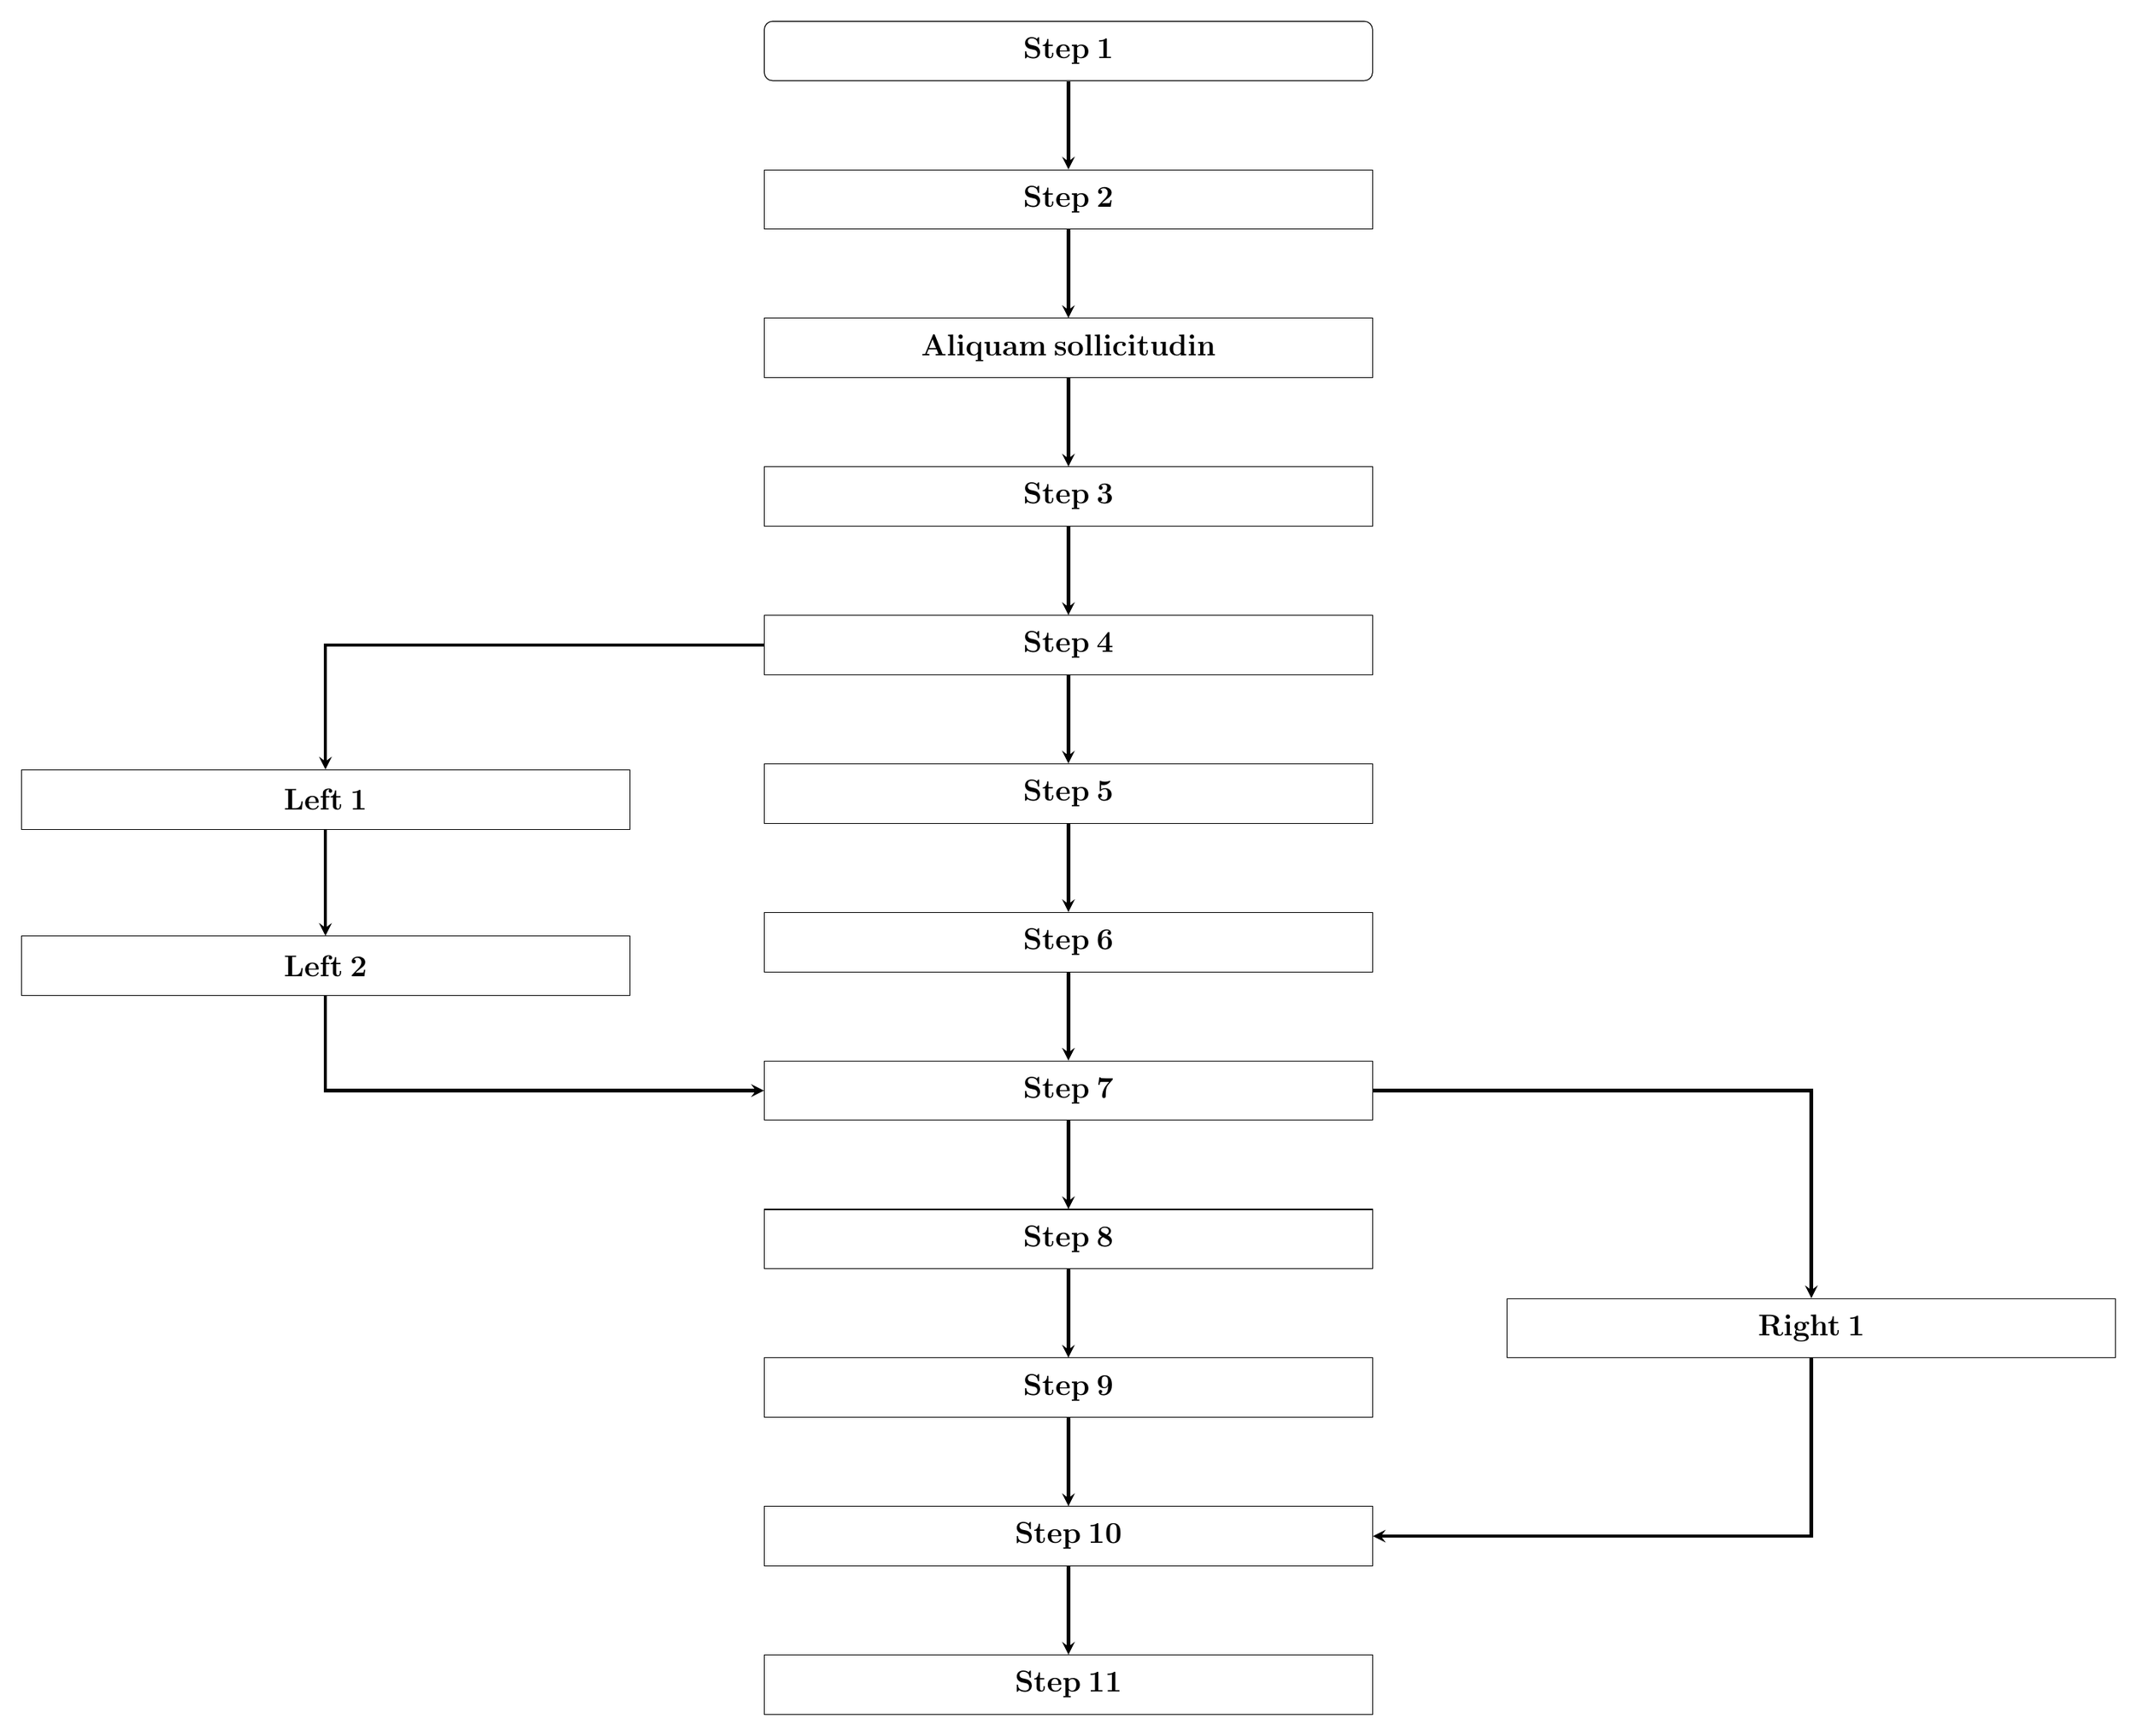
\begin{tikzpicture}[node distance=2.5cm]
                \node (start) [startstop] {\textbf{{\Large Step 1}}};
                \node (objectives) [process, below of = start] {\textbf{{\Large Step 2}}};
                \node (data_collection) [process, below of = objectives] {\textbf{{\Large Aliquam sollicitudin}}};
                \node (variables) [process, below of = data_collection] {\textbf{{\Large Step 3}}};
                \node (filter) [process, below of = variables] {\textbf{{\Large Step 4}}};

                \node (hazard) [process, below of = filter] {\textbf{{\Large Step 5}}};

                \node (cox_ph) [process, below of = hazard] {\textbf{{\Large Step 6}}};

                \node (ph_assumption) [process, below of = cox_ph] {\textbf{{\Large Step 7}}};

                \node (violated) [process, below of = ph_assumption] {\textbf{{\Large Step 8}}};

                \node (aft) [process, below of = violated] {\textbf{{\Large Step 9}}};

                \node (conclusions) [process, below of = aft] {\textbf{{\Large Step 10}}};

                 \node (policy) [process, below of = conclusions] {\textbf{{\Large Step 11}}};


% ---------------------------------------------
% All arrows (for vertical column
% ---------------------------------------------

                %  All arrows (for vertical column
                \draw [arrow] (start) -- (objectives);
                \draw [arrow] (objectives) -- (data_collection);
                \draw [arrow] (data_collection) -- (variables);
                \draw [arrow] (variables) -- (filter);
                \draw [arrow] (filter) -- (hazard);
                \draw [arrow] (hazard) -- (cox_ph);
                \draw [arrow] (cox_ph) -- (ph_assumption);
                \draw [arrow] (ph_assumption) -- (violated);
                \draw [arrow] (violated) -- (aft);
                \draw [arrow] (aft) -- (conclusions);
                \draw [arrow] (conclusions) -- (policy);
% ---------------------------------------------
% Left Division
% --------------------------------------------- 
                \node (response) [process, left of = filter, xshift=-10cm, yshift=-2.6cm] {\textbf{{\Large Left 1}}};

                \node (km_curve) [process, below of = response, yshift=-0.3cm] {\textbf{{\Large Left 2}}};
                

% ---------------------------------------------
% All arrows (for the left column)
% ---------------------------------------------

                %  All arrows (for vertical column
                \draw [arrow] (filter) -| (response);
                \draw [arrow] (response) -- (km_curve);
                \draw [arrow] (km_curve) |- (ph_assumption);

% ---------------------------------------------
% Right Division
% ---------------------------------------------   
                \node (valid) [process, right of = ph_assumption, xshift=10cm, yshift=-4cm] {\textbf{{\Large Right 1}}};

% ---------------------------------------------
% All arrows (for right column)
% ---------------------------------------------

                %  All arrows (for vertical column
                \draw [arrow] (ph_assumption) -| (valid);
                \draw [arrow] (valid) |- (conclusions);
                
            \end{tikzpicture}
        \end{adjustbox}
    \end{center}
    \caption{Study methodology.}
    \label{fig:figure3_1}
\end{figure}


% Chapter Template
---------------------------------------------------------
%	SECTION 1
%----------------------------------------------------------------------------------------
\section{Expected Results}
Write a page/two what do you want to expect from the proposed methodology…expected results?

[Write as I told in the class…] 

[Size of this section about one page]



\subsection{How to add figure}
\begin{figure}
\centering
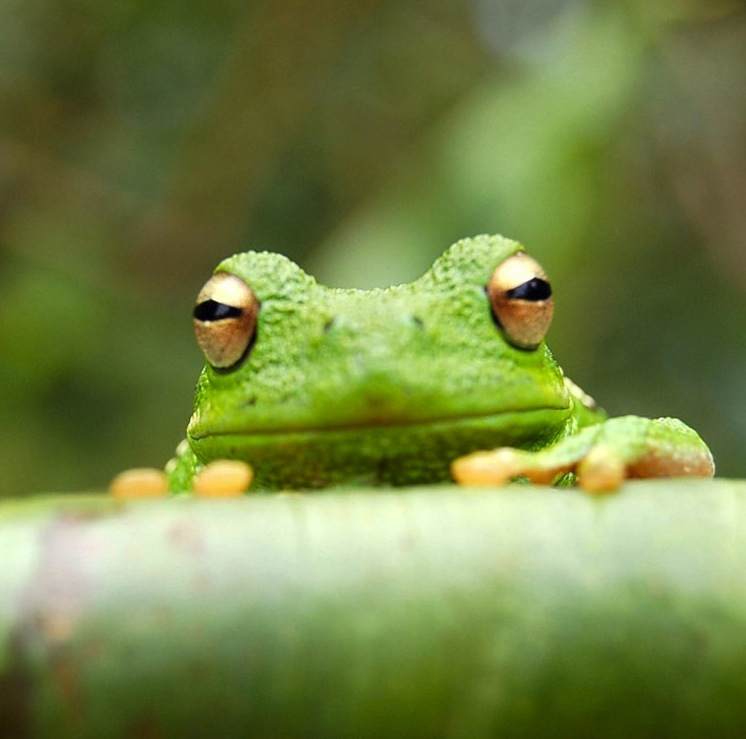
\includegraphics[width=0.3\textwidth]{Chapters/Chapter_4/frog1.jpg}
\caption{\label{fig:frog}This frog was uploaded via the file-tree menu.\cite{textbook}}
\end{figure}
\subsection{How to add table}
Use the table and tabular environments for basic tables --- see Table~\ref{tab:widgets}, for example\cite{article}. For more information, please see this help article on \href{https://www.overleaf.com/learn/latex/tables}{tables}. 
\begin{table}[ht]
\centering
\begin{tabular}{l|r}
Item & Quantity \\\hline
Widgets & 42 \\
Gadgets & 13
\end{tabular}
\caption{\label{tab:widgets}An example table.}
\end{table}

\subsection{How to add Lists}

You can make lists with automatic numbering \dots

\begin{enumerate}
\item Like this,
\item and like this.
\end{enumerate}
\dots or bullet points \dots
\begin{itemize}
\item Like this,
\item and like this.
\end{itemize}

\subsection{How to write Formula}

\LaTeX{} is great at typesetting mathematics. Let $X_1, X_2, \ldots, X_n$ be a sequence of independent and identically distributed random variables with $\text{E}[X_i] = \mu$ and $\text{Var}[X_i] = \sigma^2 < \infty$, and let
\[S_n = \frac{X_1 + X_2 + \cdots + X_n}{n}
      = \frac{1}{n}\sum_{i}^{n} X_i\]
denote their mean. Then as $n$ approaches infinity, the random variables $\sqrt{n}(S_n - \mu)$ converge in distribution to a normal $\mathcal{N}(0, \sigma^2)$.

% Chapter Template

\section{Plan of Work}
This section covers a summary of your time – plan to complete the project. Use a suitable method to represent your time – plan from Sem – VII till Sem VIII.


\subsection{Grant Chart}
\section{Conclusion}
Finally, write conclusion…about one page…
%% Chapter Template

\chapter{Introduction}\doublespacing % Main chapter title

\label{Chapter1} % Change X to a consecutive number; for referencing this chapter elsewhere, use \ref{ChapterX}

\lhead{Chapter I. \emph{Introduction}} % Change X to a consecutive number; this is for the header on each page - perhaps a shortened title

%----------------------------------------------------------------------------------------
%	SECTION 1
%----------------------------------------------------------------------------------------
\section{Introduction}
The introduction should briefly place the study in a broad context and highlight why it is important. It should define the purpose of the work and its significance. 
\begin{itemize}
    \item 
    \item 

\end{itemize}
\subsection{Objective}

\subsection{Problem Statement}




%% Chapter Template

\chapter{Literature Review}\doublespacing % Main chapter title

\label{Chapter2} % Change X to a consecutive number; for referencing this chapter elsewhere, use \ref{ChapterX}

\lhead{Chapter II. \emph{Literature Review}} % 

\section{Related Work}
This should demonstrate a sound understanding of the current state of knowledge in the field, which should critically assess previous and current work in the public domain, drawing out the major facts, views, trends, etc. (not just listing a series of literature/information sources and/or literature/ information abstracts).






 
%% Chapter Template

\chapter{Methodology}\doublespacing % Main chapter title

\label{Chapter3} % Change X to a consecutive number; for referencing this chapter elsewhere, use \ref{ChapterX}

\lhead{Chapter III. \emph{Study Methodology}} % Change X to a consecutive number; this is for the header on each page - perhaps a shortened title

%----------------------------------------------------------------------------------------
%	SECTION 1
%----------------------------------------------------------------------------------------

\section{Methodology}
This chapter presents the methodology used in conjunction with various modeling techniques, including non-parametric, semi-parametric, and parametric models.
\subsection{How to add equation \ref{Eq3_1}.}
% Equation
\begin{equation}
e = \lim_{n\to\infty} \left(1+\frac{1}{n}\right)^n
\label{Eq3_1}
\end{equation} 

\begin{align}
	x^2 -25 &= 0 \nonumber \\
	x^2 &= 25 \nonumber \\
	\therefore \Aboxed{x &= 5}
 \label{Eq3_2}
\end{align}



\begin{multline}
	f(x) = 4xy^2 + 3x^3 - 2xy + 25x^3y^3 + 3xy - 4x^6y^6 + 3xy^2 - 2y^3\\ + a^3b^3c^4 + 3x^3 - 2xy + 25x^3y^3 + 3xy\\ - 4x^6y^6 + 3xy^2 - 2y^3 + a^3b^3c^4
\label{Eq3_3}
\end{multline}



\section{Models and Algorithms}
% adjustbox is used to limit the figure inside page
% -- means normal arrow
%  -| horizontal then vertical arrow
%  |- vertical then horizontal arrow


\begin{figure}[!ht]

    \begin{center}
        \begin{adjustbox}{max height=0.8\textheight, center, width=0.6\textwidth}
            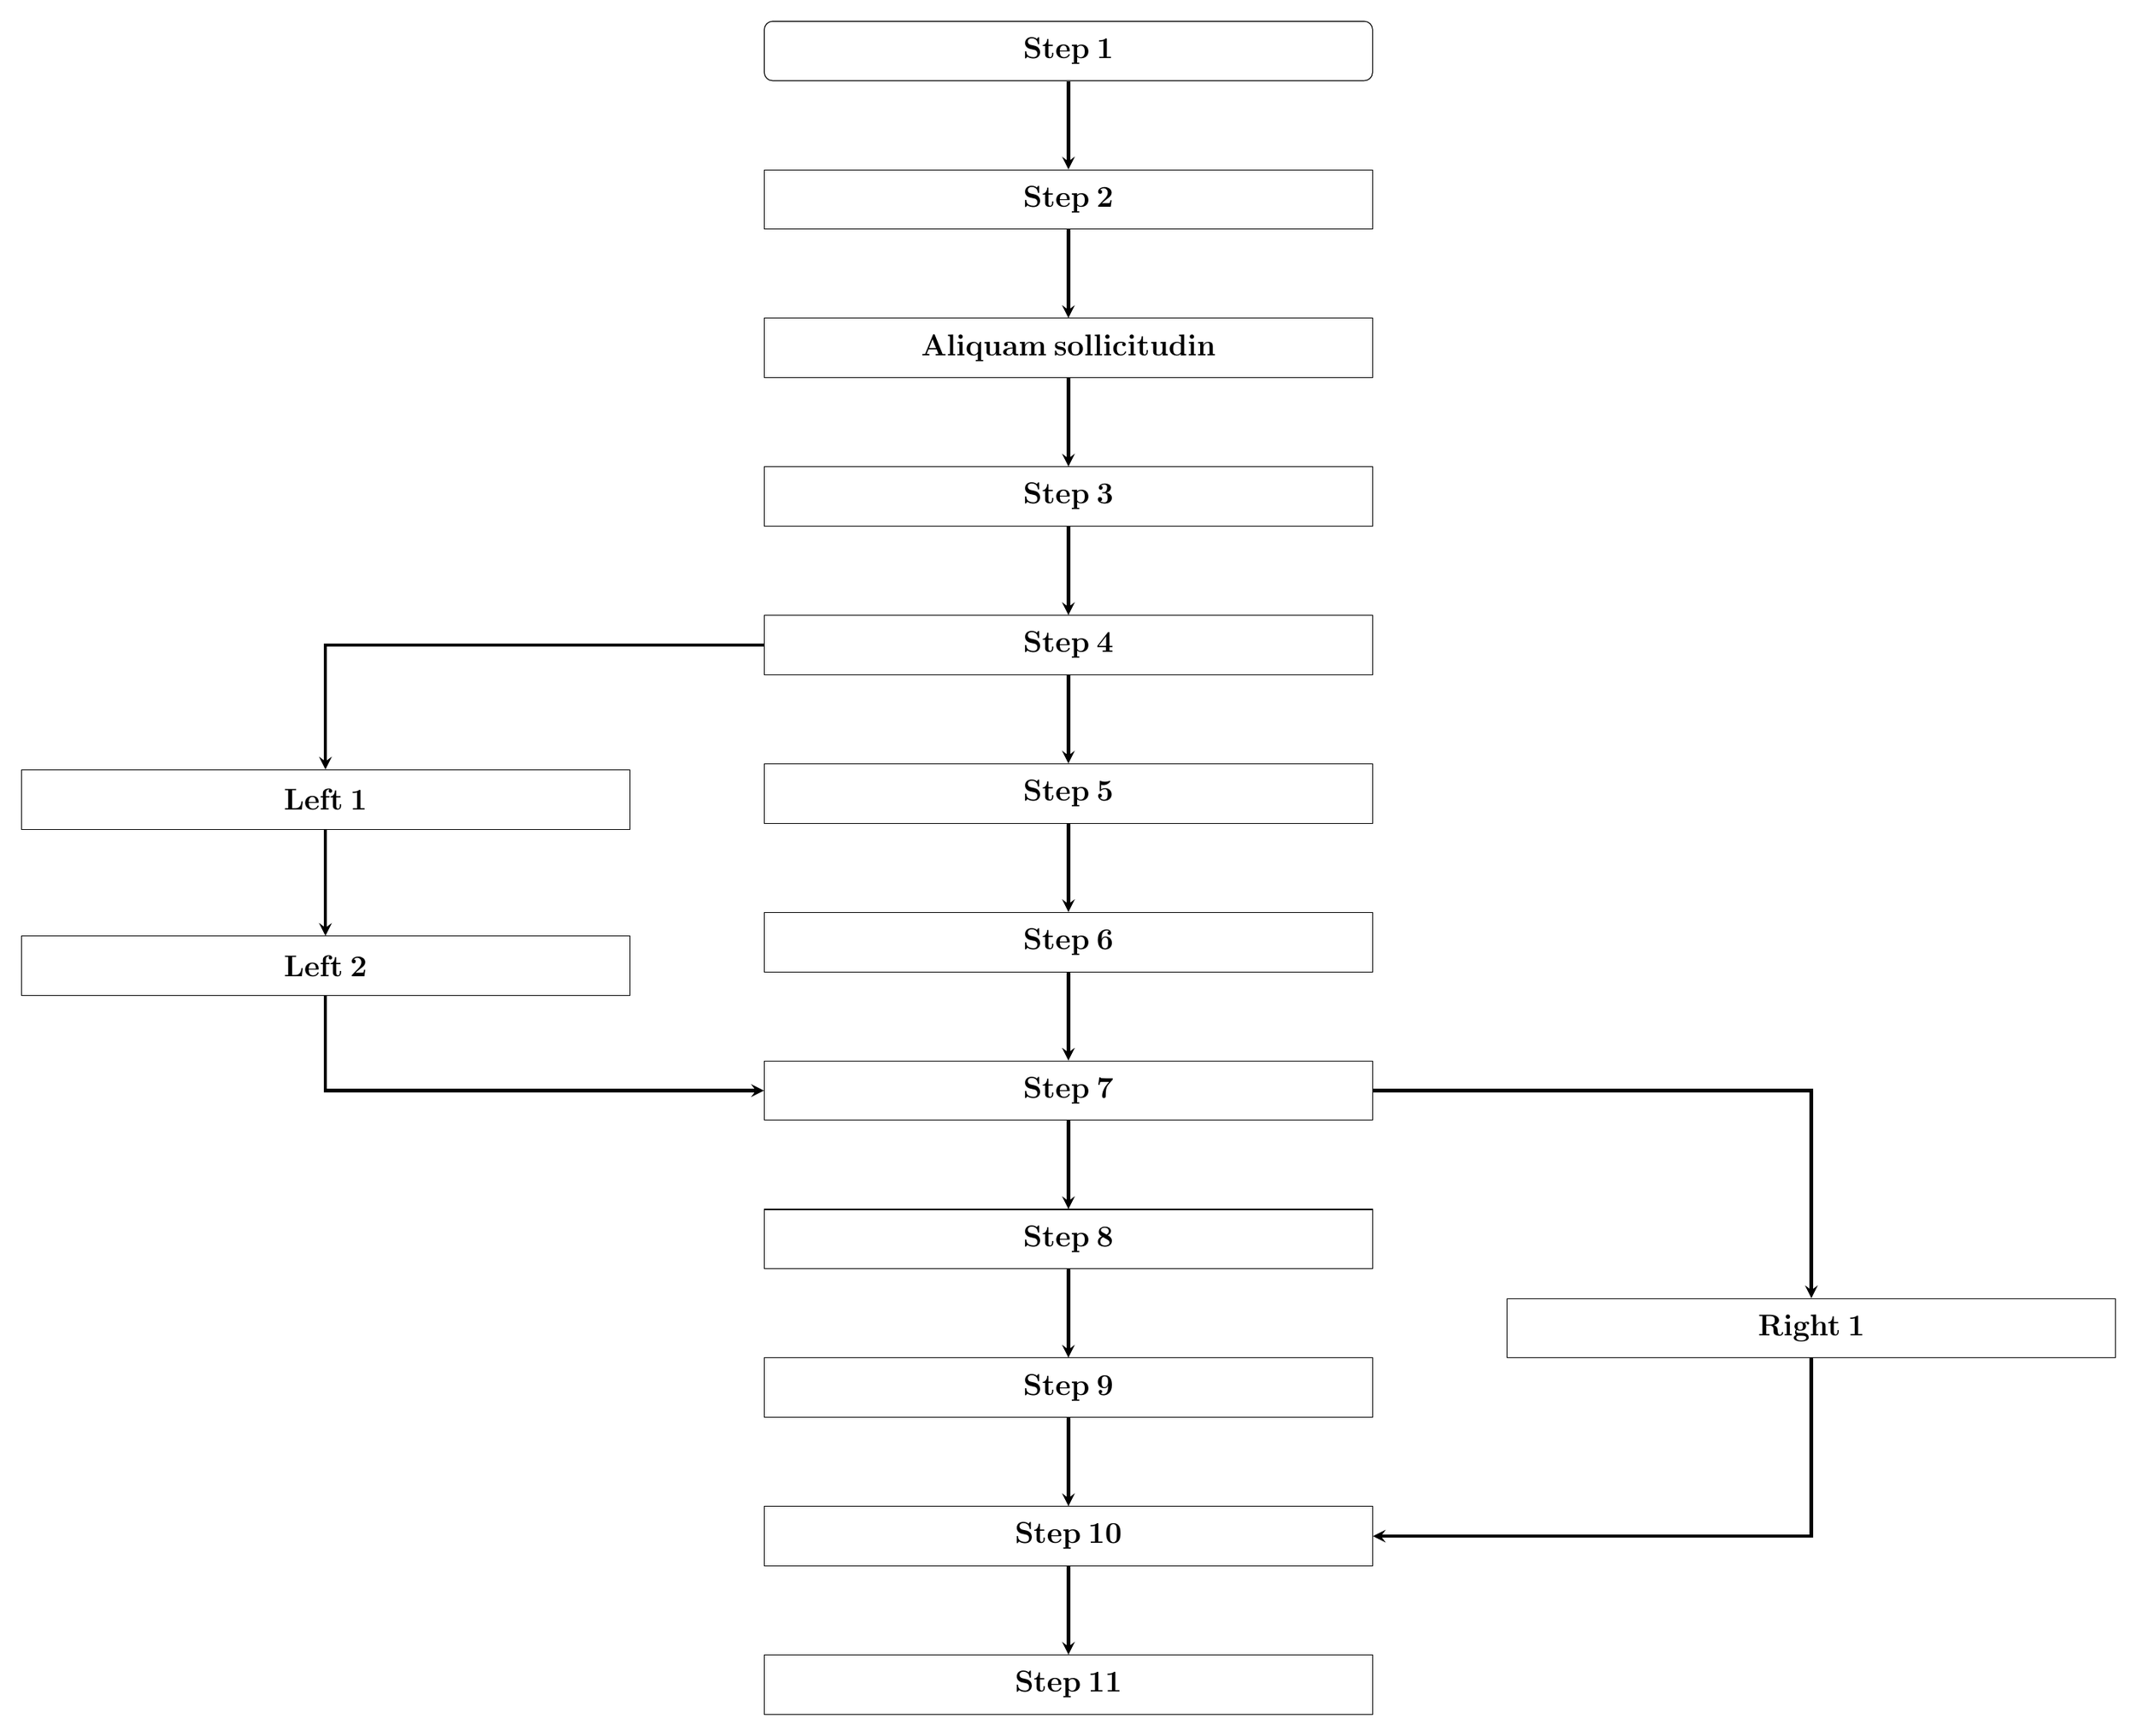
\begin{tikzpicture}[node distance=2.5cm]
                \node (start) [startstop] {\textbf{{\Large Step 1}}};
                \node (objectives) [process, below of = start] {\textbf{{\Large Step 2}}};
                \node (data_collection) [process, below of = objectives] {\textbf{{\Large Aliquam sollicitudin}}};
                \node (variables) [process, below of = data_collection] {\textbf{{\Large Step 3}}};
                \node (filter) [process, below of = variables] {\textbf{{\Large Step 4}}};

                \node (hazard) [process, below of = filter] {\textbf{{\Large Step 5}}};

                \node (cox_ph) [process, below of = hazard] {\textbf{{\Large Step 6}}};

                \node (ph_assumption) [process, below of = cox_ph] {\textbf{{\Large Step 7}}};

                \node (violated) [process, below of = ph_assumption] {\textbf{{\Large Step 8}}};

                \node (aft) [process, below of = violated] {\textbf{{\Large Step 9}}};

                \node (conclusions) [process, below of = aft] {\textbf{{\Large Step 10}}};

                 \node (policy) [process, below of = conclusions] {\textbf{{\Large Step 11}}};


% ---------------------------------------------
% All arrows (for vertical column
% ---------------------------------------------

                %  All arrows (for vertical column
                \draw [arrow] (start) -- (objectives);
                \draw [arrow] (objectives) -- (data_collection);
                \draw [arrow] (data_collection) -- (variables);
                \draw [arrow] (variables) -- (filter);
                \draw [arrow] (filter) -- (hazard);
                \draw [arrow] (hazard) -- (cox_ph);
                \draw [arrow] (cox_ph) -- (ph_assumption);
                \draw [arrow] (ph_assumption) -- (violated);
                \draw [arrow] (violated) -- (aft);
                \draw [arrow] (aft) -- (conclusions);
                \draw [arrow] (conclusions) -- (policy);
% ---------------------------------------------
% Left Division
% --------------------------------------------- 
                \node (response) [process, left of = filter, xshift=-10cm, yshift=-2.6cm] {\textbf{{\Large Left 1}}};

                \node (km_curve) [process, below of = response, yshift=-0.3cm] {\textbf{{\Large Left 2}}};
                

% ---------------------------------------------
% All arrows (for the left column)
% ---------------------------------------------

                %  All arrows (for vertical column
                \draw [arrow] (filter) -| (response);
                \draw [arrow] (response) -- (km_curve);
                \draw [arrow] (km_curve) |- (ph_assumption);

% ---------------------------------------------
% Right Division
% ---------------------------------------------   
                \node (valid) [process, right of = ph_assumption, xshift=10cm, yshift=-4cm] {\textbf{{\Large Right 1}}};

% ---------------------------------------------
% All arrows (for right column)
% ---------------------------------------------

                %  All arrows (for vertical column
                \draw [arrow] (ph_assumption) -| (valid);
                \draw [arrow] (valid) |- (conclusions);
                
            \end{tikzpicture}
        \end{adjustbox}
    \end{center}
    \caption{Study methodology.}
    \label{fig:figure3_1}
\end{figure}


%% Chapter Template

\chapter{Expected Results}\doublespacing % Main chapter title

\label{Chapter4} % Change X to a consecutive number; for referencing this chapter elsewhere, use \ref{ChapterX}

\lhead{Chapter IV. \emph{Expected Results}} % Change X to a consecutive number; this is for the header on each page - perhaps a shortened title
 % Change X to a consecutive number; this is for the header on each page - perhaps a shortened title
%----------------------------------------------------------------------------------------
%	SECTION 1
%----------------------------------------------------------------------------------------
\section{Experimental Result}




\subsection{How to add figure}
\begin{figure}
\centering
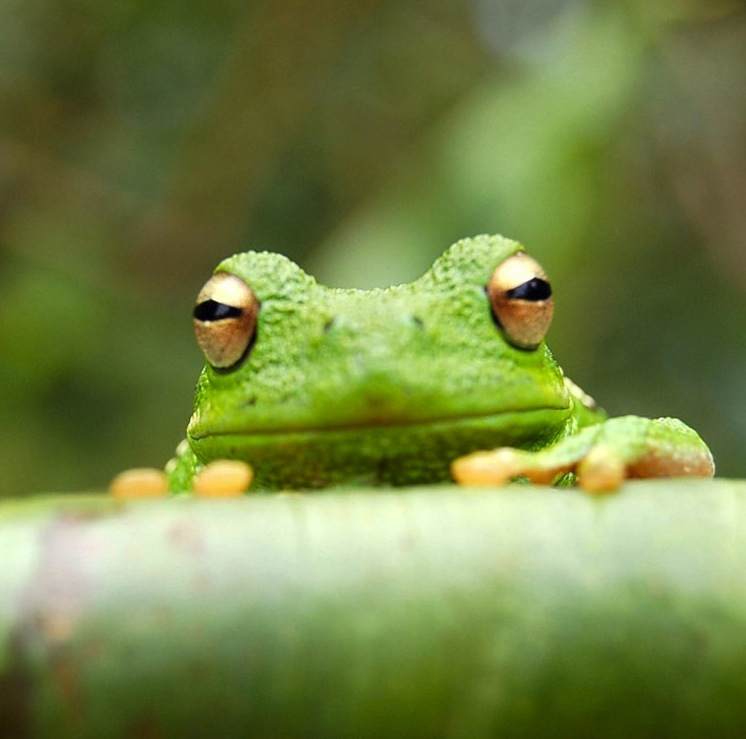
\includegraphics[width=0.3\textwidth]{Chapters/Chapter_4/frog1.jpg}
\caption{\label{fig:frog}This frog was uploaded via the file-tree menu.\cite{textbook}}
\end{figure}
\subsection{How to add table}
Use the table and tabular environments for basic tables --- see Table~\ref{tab:widgets}, for example\cite{article}. For more information, please see this help article on \href{https://www.overleaf.com/learn/latex/tables}{tables}. 

\begin{table}[ht]
\centering
\begin{tabular}{l|r}
Item & Quantity \\\hline
Widgets & 42 \\
Gadgets & 13
\end{tabular}
\caption{\label{tab:widgets}An example table.}
\end{table}

\subsection{How to add Lists}

You can make lists with automatic numbering \dots

\begin{enumerate}
\item Like this,
\item and like this.
\end{enumerate}
\dots or bullet points \dots
\begin{itemize}
\item Like this,
\item and like this.
\end{itemize}

\subsection{How to write Formula}

\LaTeX{} is great at typesetting mathematics. Let $X_1, X_2, \ldots, X_n$ be a sequence of independent and identically distributed random variables with $\text{E}[X_i] = \mu$ and $\text{Var}[X_i] = \sigma^2 < \infty$, and let
\[S_n = \frac{X_1 + X_2 + \cdots + X_n}{n}
      = \frac{1}{n}\sum_{i}^{n} X_i\]
denote their mean. Then as $n$ approaches infinity, the random variables $\sqrt{n}(S_n - \mu)$ converge in distribution to a normal $\mathcal{N}(0, \sigma^2)$.





%%%%%%%%%%%%%%%%% Changes%%%%%%%%%%%%%%%%%%%%%%%%














































 
%% Chapter Template

\chapter{Conclusion}\doublespacing % Main chapter title


\section{Conclusion}



%%%%%%%%%%%%%%%%% Changes%%%%%%%%%%%%%%%%%%%%%%%%




\section{Grant Chart}










































 
% \input{Chapters/Chapter7} 





\clearpage % Start a new page
%----------------------------------------------------------------------------------------
%	THESIS CONTENT - APPENDICES
%----------------------------------------------------------------------------------------

\addtocontents{toc}{\vspace{2em}} % Add a gap in the Contents, for aesthetics

\appendix % Cue to tell LaTeX that the following 'chapters' are Appendices
% Appendix Template

%\chapter{Appendix} % Main appendix title




% Include the appendices of the thesis as separate files from the Appendices folder
% Uncomment the lines as you write the Appendices

%\input{Appendices/AppendixA}
% \input{Appendices/AppendixC}
%\input{Appendices/AppendixD}

\addtocontents{toc}{\vspace{2em}} % Add a gap in the Contents, for aesthetics

%\backmatter

%----------------------------------------------------------------------------------------
%	BIBLIOGRAPHY
%----------------------------------------------------------------------------------------

\label{References}
\lhead{\emph{References}} % Change the page header to say "Bibliography"

\renewcommand\bibname{References}
\begin{thebibliography}{99}
\bibitem{textbook}

M. Abramowitz and I. A. Stegun, Eds., \textit{Handbook of Mathematical Functions} (Applied Mathematics Series 55). Washington, DC, USA: NBS, 1964, pp. 32$-$33.

\bibitem{Book chapter}

 T. Ogura, “Electronic government and surveillance-oriented society,” in \emph{Theorizing Surveillance: The Panopticon and Beyond}. Cullompton, U.K.: Willan, 2006, ch. 13, pp. 270$-$295.

\bibitem{article}

K. A. Nelson, R. J. Davis, D. R. Lutz, and W. Smith, “Optical generation of
tunable ultrasonic waves,” \textit{Journal of Applied Physics}, vol. 53, no.2, pp. 1144$-$1149, 2002.

\bibitem{Conference papers}

S. P. Bingulac, “On the compatibility of adaptive controllers,” in \textit{Proc. of 4th Annual Conference on Circuit Systems Theory}, New York, NY, USA, 1994, pp. 8$-$16.

\bibitem{Website}
$-$, Online Available at: https://nli.vnunet.com/news/1116995. [Accessed on May, 2023].

\bibitem{Dataset}

S. Ansolabehere, M. Palmer, and A. Lee. “Precinct-level election data. V1.” January 20, 2014. Distributed by Harvard Election Data Archive, Online Available at: https://link. [Accessed on May, 2023] 

\end{thebibliography}


\end{document}  
